% ROS Node Graph — TIAGo Door-Opening System
\documentclass[border=10pt]{standalone}
\usepackage{tikz}
\usetikzlibrary{positioning, fit, backgrounds, arrows.meta, calc}
\usepackage[T1]{fontenc}
\usepackage{lmodern}

\newcommand{\pkglbl}[1]{{\fontsize{12}{8}\selectfont\sffamily\color{black!50}#1}}

\colorlet{cBLUE}{blue!20}
\colorlet{cGRAY_DARK}{gray!20}
\colorlet{cGRAY_LIGHT}{gray!8}
\colorlet{cWHITE}{white}


\begin{document}
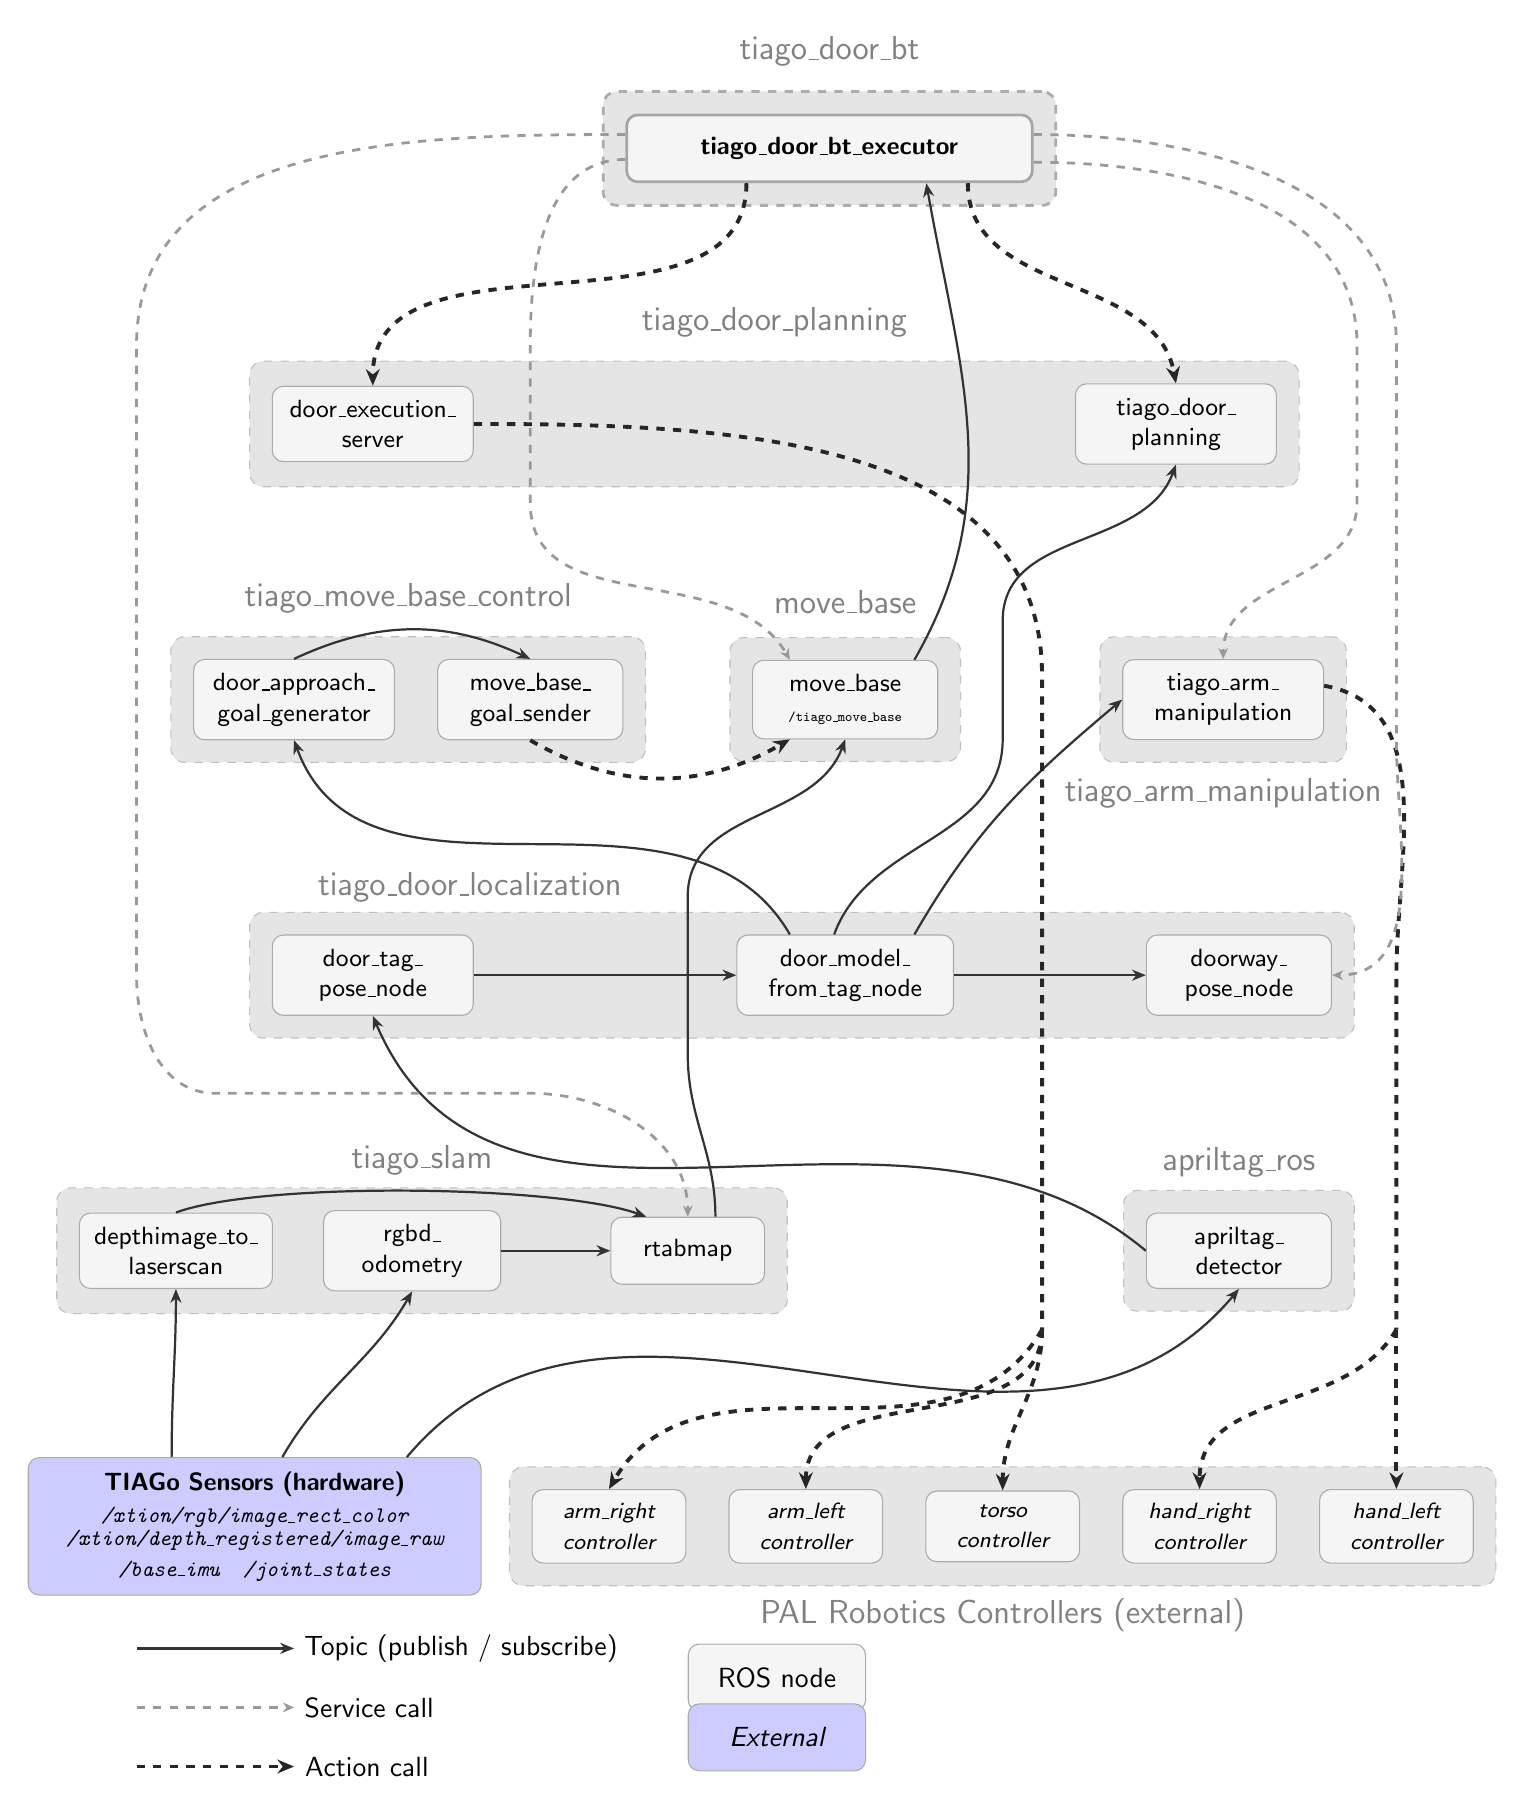
\begin{tikzpicture}[
  N/.style={draw=gray!65, rounded corners=4pt, align=center,
            inner sep=5pt, minimum height=0.85cm, font=\small\sffamily},
  E/.style={N, font=\small\sffamily\itshape},
  topic/.style={-{Stealth[length=5pt,width=4pt]}, thick, draw=black!80},
  srv/.style={-{Stealth[length=4pt,width=3.5pt]}, dashed, draw=black!40, line width=1.0pt},
  act/.style={-{Stealth[length=6pt,width=5pt]}, dashed, line width=1.4pt,
              draw=black!85},
  trunk/.style={dashed, line width=1.4pt, draw=black!85},
  L/.style={font=\fontsize{5}{6}\selectfont\ttfamily,
            fill=white, inner sep=0.8pt, text=black!65, align=left},
  grp/.style={draw=gray!50, dashed, rounded corners=5pt,
              inner sep=8pt, fill=#1},
]

%  ROW 0 (y=0)  Sensors  +  Hardware Controllers
\node[E, fill=cBLUE, text width=5.4cm] (sensors) at (1.5, 0) {
  \textbf{TIAGo Sensors (hardware)}\\[3pt]
  \fontsize{8}{7}\selectfont\ttfamily
  /xtion/rgb/image\_rect\_color\\
  /xtion/depth\_registered/image\_raw\\
  /base\_imu\quad /joint\_states
};

\node[E, fill=cGRAY_LIGHT, text width=1.6cm] (ca_r)    at ( 6, 0)
  {\fontsize{8}{8}\selectfont arm\_right\\ controller};
\node[E, fill=cGRAY_LIGHT, text width=1.6cm] (ca_l)    at (8.5, 0)
  {\fontsize{8}{8}\selectfont arm\_left\\ controller};
\node[E, fill=cGRAY_LIGHT, text width=1.6cm] (c_torso) at (11.0, 0)
  {\fontsize{8}{8}\selectfont torso\\ controller};
\node[E, fill=cGRAY_LIGHT, text width=1.6cm] (ch_r)    at (13.5, 0)
  {\fontsize{8}{8}\selectfont hand\_right\\ controller};
\node[E, fill=cGRAY_LIGHT, text width=1.6cm] (ch_l)    at (16.0, 0)
  {\fontsize{8}{8}\selectfont hand\_left\\ controller};

\begin{pgfonlayer}{background}
  \node[grp=cGRAY_DARK, fit=(ca_r)(ca_l)(c_torso)(ch_r)(ch_l)] (grp_ctrl) {};
\end{pgfonlayer}
\node[below=20pt of grp_ctrl.south, anchor=south]
  {\pkglbl{PAL Robotics Controllers (external)}};

%  ROW 1 (y=4.2)  SLAM  +  AprilTag Detection
\node[N, fill=cGRAY_LIGHT, text width=2.1cm] (dep2scan) at (0.5, 3.5)
  {depthimage\_to\_\\laserscan};
\node[N, fill=cGRAY_LIGHT, text width=1.9cm] (rgbd)     at (3.5, 3.5)
  {rgbd\_\\odometry};
\node[N, fill=cGRAY_LIGHT, text width=1.6cm] (rtab)     at (7, 3.5)
  {rtabmap};
\node[N, fill=cGRAY_LIGHT, text width=2.0cm] (april)   at (14, 3.5)
  {apriltag\_\\detector};

\begin{pgfonlayer}{background}
  \node[grp=cGRAY_DARK, fit=(dep2scan)(rgbd)(rtab)] (grp_slam) {};
  \node[grp=cGRAY_DARK, fit=(april)]               (grp_april) {};
\end{pgfonlayer}
\node[above=1pt of grp_slam.north,  anchor=south] {\pkglbl{tiago\_slam}};
\node[above=1pt of grp_april.north, anchor=south] {\pkglbl{apriltag\_ros}};

%  ROW 2 (y=8.4)  Door Localization
\node[N, fill=cGRAY_LIGHT, text width=2.2cm] (tagpose)   at ( 3.0, 7)
  {door\_tag\_\\pose\_node};
\node[N, fill=cGRAY_LIGHT, text width=2.4cm] (doormodel) at (9.0, 7)
  {door\_model\_\\from\_tag\_node};
\node[N, fill=cGRAY_LIGHT, text width=2.0cm] (doorway)   at (14, 7)
  {doorway\_\\pose\_node};

\begin{pgfonlayer}{background}
  \node[grp=cGRAY_DARK, fit=(tagpose)(doormodel)(doorway)] (grp_loc) {};
\end{pgfonlayer}
\node[above=1pt of grp_loc.north, left=120pt of grp_loc.north, anchor=south]
  {\pkglbl{tiago\_door\_localization}};

%  ROW 3 (y=12.6)  Navigation  +  Arm Manipulation
\node[N, fill=cGRAY_LIGHT, text width=2.2cm] (goalgen)  at (2, 10.5)
  {door\_approach\_\\goal\_generator};
\node[N, fill=cGRAY_LIGHT, text width=2.0cm] (goalsend) at (5.0, 10.5)
  {move\_base\_\\goal\_sender};
\node[N, fill=cGRAY_LIGHT, text width=2.0cm] (mb)       at (9, 10.5)
  {move\_base\\{\fontsize{5}{6}\selectfont\ttfamily /tiago\_move\_base}};
\node[N, fill=cGRAY_LIGHT, text width=2.2cm] (arm)      at (13.8, 10.5)
  {tiago\_arm\_\\manipulation};

\begin{pgfonlayer}{background}
  \node[grp=cGRAY_DARK, fit=(goalgen)(goalsend)] (grp_nav) {};
  \node[grp=cGRAY_DARK,  fit=(mb)]               (grp_mb)  {};
  \node[grp=cGRAY_DARK, fit=(arm)]              (grp_arm) {};
\end{pgfonlayer}
\node[above=5pt of grp_nav.north, anchor=south]
  {\pkglbl{tiago\_move\_base\_control}};
\node[above=5pt of grp_mb.north,  anchor=south] {\pkglbl{move\_base}};
\node[below=20pt of grp_arm.south, anchor=south]
  {\pkglbl{tiago\_arm\_manipulation}};

%  ROW 4 (y=16.8)  Planning & Execution
\node[N, fill=cGRAY_LIGHT, text width=2.2cm] (planner)  at (13.2, 14.0)
  {tiago\_door\_\\planning};
\node[N, fill=cGRAY_LIGHT, text width=2.2cm] (executor) at (3, 14.0)
  {door\_execution\_\\server};

\begin{pgfonlayer}{background}
  \node[grp=cGRAY_DARK, fit=(planner)(executor)] (grp_plan) {};
\end{pgfonlayer}
\node[above=5pt of grp_plan.north, anchor=south]
  {\pkglbl{tiago\_door\_planning}};

%  ROW 5 (y=21.0)  Behavior Tree
\node[N, fill=cGRAY_LIGHT, draw=gray!70, line width=1pt, text width=4.8cm]
  (bt) at (8.8, 17.5) {\textbf{tiago\_door\_bt\_executor}};

\begin{pgfonlayer}{background}
  \node[grp=cGRAY_DARK, draw=gray!65, line width=1pt, fit=(bt)] (grp_bt) {};
\end{pgfonlayer}
\node[above=5pt of grp_bt.north, anchor=south] {\pkglbl{tiago\_door\_bt}};

%  TOPIC ARROWS  (upward data flow)

% sensors -> depthimage_to_laserscan
\draw[topic] ([xshift=-30pt]sensors.north) to[out=90, in=270] (dep2scan.south);

% sensors -> rgbd_odometry
\draw[topic] ([xshift=10pt]sensors.north) to[out=60, in=240] (rgbd.south);

% sensors -> apriltag_detector
\draw[topic] ([xshift=55pt]sensors.north) to[out=50, in=230] (april.south);

% depthimage_to_laserscan -> rtabmap
\draw[topic] (dep2scan.north) to[out=20, in=160, looseness=0.5] ([xshift=-15pt]rtab.north);

% rgbd_odometry -> rtabmap
\draw[topic] (rgbd.east) to[out=0, in=180] (rtab.west);

% apriltag -> tag_pose_node
\draw[topic] (april.west) to[out=140, in=293] (tagpose.south);

% tag_pose_node -> door_model_from_tag_node
\draw[topic] (tagpose.east) to[out=0, in=180] (doormodel.west);

% door_model -> doorway_pose_node
\draw[topic] (doormodel.east) to[out=0, in=180] (doorway.west);

% door_model -> goal_generator
\draw[topic] ([xshift=-20pt]doormodel.north) to[out=120, in=290] (goalgen.south);

% door_model -> planner
\draw[topic] ([xshift=-4pt]doormodel.north) to[out=70, in=270] (11, 10) to[out=90, in=270] (11, 11.5) to[out=90, in=250] (planner.south);

% door_model -> arm_manipulation
\draw[topic] ([xshift=25pt]doormodel.north) to[out=60, in=220] (arm.west);

% rtabmap -> move_base  (/map)
\draw[topic] ([xshift=10pt]rtab.north) to[out=90, in=270] (7,6) to[out=90, in=270] (7,8) to[out=90, in=250] ([xshift=-00pt]mb.south);

% goal_generator -> goal_sender
\draw[topic] (goalgen.north) to[out=25, in=155] (goalsend.north);

% move_base -> bt  (status topic)
\draw[topic] ([xshift=25pt]mb.north) to[out=60, in=280] ([xshift=35pt]bt.south);

%  ACTION ARROWS  (thick dashed)

% goal_sender -> move_base
\draw[act] (goalsend.south) to[out=330, in=210] ([xshift=-20pt]mb.south);

% BT -> planner
\draw[act] ([xshift=50pt]bt.south) to[out=270, in=100] (planner.north);

% BT -> executor
\draw[act] ([xshift=-30pt]bt.south) to[out=270, in=90] (executor.north);

% executor -> arm/torso controllers
\draw[trunk] (executor.east) to[out=0, in=90] (11.5, 10.8) to[out=270, in=90] (11.5, 2.5);
\draw[act] (11.5, 2.5) to[out=240, in=60] (ca_r.north);
\draw[act] (11.5, 2.5) to[out=270, in=90] (ca_l.north);
\draw[act] (11.5, 2.5) to[out=270, in=90] (c_torso.north);

% arm_manip -> hand controllers
\draw[trunk] ([yshift=5pt]arm.east) to[out=350, in=90] (16.0, 7.0) to[out=270, in=90] (16, 2.5);
\draw[act] (16.0, 2.5) to[out=240, in=90] (ch_r.north);
\draw[act] (16.0, 2.5) to[out=270, in=90] (ch_l.north);

%  SERVICE ARROWS  (thin dashed)

% BT -> rtabmap/set_mode_*
\draw[srv] ([yshift=5pt]bt.west) to[out=180, in=90] (0.0, 15) to[out=270, in=90] (0.0, 7.0) to[out=270, in=180] (1.0, 5.5)
  to[out=0, in=180] (5.0, 5.5) to[out=0, in=90] (rtab.north);

% BT -> move_base/clear_costmaps
\draw[srv]
  ([yshift=-4pt]bt.west) to[out=180, in=90] (5, 15) to[out=270, in=90] (5, 13) to[out=270, in=120] ([xshift=-20pt]mb.north);

% BT -> doorway_pose_node/freeze
\draw[srv]
  ([yshift=5pt]bt.east) to[out=0, in=90] (16, 15) to[out=270, in=90] (16, 10) to[out=270, in=0] (doorway.east);

% BT -> arm_manipulation services
\draw[srv]
  ([yshift=-5pt]bt.east) to[out=0, in=90] (15.5, 15) to[out=270, in=90] (15.5, 13) to[out=270, in=90] (arm.north);

%  LEGEND
\begin{scope}[shift={(0, -2.3)}]
  \draw[topic] (0.0, 0.75) -- ++(2.0,0)
    node[right, font=\fontsize{10}{10}\selectfont\sffamily]
      {Topic (publish / subscribe)};
  \draw[srv]   (0.0, 0.00) -- ++(2.0,0)
    node[right, font=\fontsize{10}{10}\selectfont\sffamily]{Service call};
  \draw[act]   (0.0,-0.75) -- ++(2.0,0)
    node[right, font=\fontsize{10}{10}\selectfont\sffamily]{Action call};
  \node[N, fill=cGRAY_LIGHT, text width=1.9cm, anchor=west,
        font=\fontsize{10}{10}\selectfont\sffamily]
    at (7.0, 0.38) {ROS node};
  \node[E, fill=cBLUE, text width=1.9cm, anchor=west,
        font=\fontsize{10}{10}\selectfont\sffamily\itshape]
    at (7.0,-0.38) {External};
\end{scope}

\end{tikzpicture}
\end{document}
